\chapter{Software}
\label{atomics}

\begin{figure*}[!t]
	\centering
	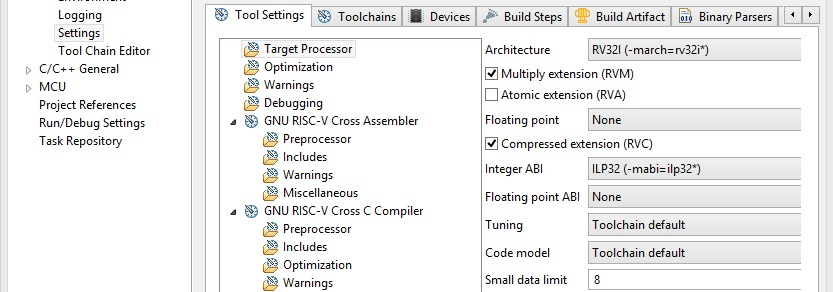
\includegraphics[width=7in]{figs/setting}
	\caption{Compiler settings.}
	\label{Compiler_setting}
\end{figure*}

As the project's name might indicate, the programming of the system can be done using processing in the Arduino-style. The Arduissimo IDE is not part of this release but it is planned to have this included in version v0.2. 

As of now the system can be programmed using the Freedom Studio framework from SiFive. Figure \ref{Compiler_setting} shows the recommended compiler settings.

Each thread on a core shares the same program memory and the same data memory. This is why the provided examples are compiled as a single program. It is important to know that all threads potentionally use the same stack, which can be problematic, unless the stack pointer is taken care of.

In the Freedom Studio projects that come with this release, the project's name postfix (''\_0'', ..., ''\_3'') indicate, on which core the code is executed (see Figure \ref{postfix}). Compiling the projects always results in the error message, that ''elf'' execution fails. The ''elf'' to ''hex'' conversion is then done seperately by executing the relevant Makefile command. The right command in the Makefile copies the relevant ''elf'' file into a ''work'' directory, and from there it is converted into ''hex''. This example is self explaining:

\begin{figure*}[!t]
	\centering
	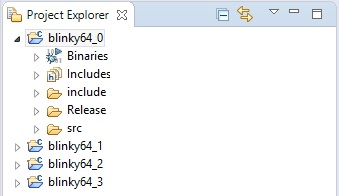
\includegraphics[width=4in]{figs/projects_postfix}
	\caption{Project's postfix indicate individual core.}
	\label{postfix}
\end{figure*}

\vspace{1in}
gsm\_32 :\\
\indent \space\space\space cd ../tests/chstone/gsm/work ;\\
\indent \space\space\space cp ../gsm\_ws\_rv32imc/gsm/Release/gsm.elf . ;\\
\indent \space\space\space riscv64-unknown-elf-objdump.exe -S gsm.elf \textgreater\space main.disasm ;\\
\indent \space\space\space riscv64-unknown-elf-objcopy.exe -j.text -O verilog gsm.elf main.hex ;\\
\indent \space\space\space riscv64-unknown-elf-objcopy.exe -j.data -O verilog gsm.elf data.hex

In the next chapters, the downloading of a ''hex'' file to the ARTY board is discussed.

